\documentclass[10pt]{beamer}
\usepackage{amsmath}
\usepackage{mathtools}
\usepackage{multimedia}
\usepackage{hyperref}


\usefonttheme{professionalfonts} % using non standard fonts for beamer
\usefonttheme{serif} % default family is serif
%\documentclass[12pt]{beamerthemeSam.sty}
\usepackage{epsf}
%\usepackage{pstricks}
%\usepackage[orientation=portrait,size=A4]{beamerposter}
\geometry{paperwidth=160mm,paperheight=120mm}
%DT favorite definitions
\def\LL{\left\langle}	% left angle bracket
\def\RR{\right\rangle}	% right angle bracket
\def\LP{\left(}		% left parenthesis
\def\RP{\right)}	% right parenthesis
\def\LB{\left\{}	% left curly bracket
\def\RB{\right\}}	% right curly bracket
\def\PAR#1#2{ {{\partial #1}\over{\partial #2}} }
\def\PARTWO#1#2{ {{\partial^2 #1}\over{\partial #2}^2} }
\def\PARTWOMIX#1#2#3{ {{\partial^2 #1}\over{\partial #2 \partial #3}} }

\def\rightpartial{{\overrightarrow\partial}}
\def\leftpartial{{\overleftarrow\partial}}
\def\diffpartial{\buildrel\leftrightarrow\over\partial}

\def\BC{\begin{center}}
\def\EC{\end{center}}
\def\BN{\begin{enumerate}}
\def\EN{\end{enumerate}}
\def\BI{\begin{itemize}}
\def\EI{\end{itemize}}
\def\BE{\begin{displaymath}}
\def\EE{\end{displaymath}}
\def\BEA{\begin{eqnarray*}}
\def\EEA{\end{eqnarray*}}
\def\BNEA{\begin{eqnarray}}
\def\ENEA{\end{eqnarray}}
\def\EL{\nonumber\\}

\newcommand{\etal}{{\it et al.}}
\newcommand{\gbeta}{6/g^2}
\newcommand{\la}[1]{\label{#1}}
\newcommand{\ie}{{\em i.e.\ }}
\newcommand{\eg}{{\em e.\,g.\ }}
\newcommand{\cf}{cf.\ }
\newcommand{\etc}{etc.\ }
\newcommand{\atantwo}{{\rm atan2}}
\newcommand{\Tr}{{\rm Tr}}
\newcommand{\dt}{\Delta t}
\newcommand{\op}{{\cal O}}
\newcommand{\msbar}{{\overline{\rm MS}}}
\def\chpt{\raise0.4ex\hbox{$\chi$}PT}
\def\schpt{S\raise0.4ex\hbox{$\chi$}PT}
\def\MeV{{\rm Me\!V}}
\def\GeV{{\rm Ge\!V}}

%AB: my color definitions
%\definecolor{mygarnet}{rgb}{0.445,0.184,0.215}
%\definecolor{mygold}{rgb}{0.848,0.848,0.098}
%\definecolor{myg2g}{rgb}{0.647,0.316,0.157}
\definecolor{A}{rgb}{1.0,0.3,0.3}
\definecolor{B}{rgb}{0.0,1.0,0.0}
\definecolor{C}{rgb}{1.0,1.0,0.0}
\definecolor{D}{rgb}{0.5,0.5,1.0}
\definecolor{E}{rgb}{0.7,0.7,0.7}
\definecolor{abtitlecolor}{rgb}{1.0,1.0,1.0}
\definecolor{absecondarycolor}{rgb}{0.0,0.416,0.804}
\definecolor{abprimarycolor}{rgb}{1.0,0.686,0.0}
\definecolor{Red}           {rgb}{1,0.4,0.4}
\definecolor{Grey}          {cmyk}{.7,.7,.7,0}
\definecolor{Blue}          {cmyk}{1,1,0,0}
\definecolor{Green}         {cmyk}{1,0,1,0}
\definecolor{Brown}         {cmyk}{0,0.81,1,0.60}
\definecolor{Silver}        {rgb}{0.95,0.9,1.0}
\definecolor{Sky}           {rgb}{0.07,0.0,0.2}
\definecolor{Darkbrown}     {rgb}{0.4,0.3,0.2}
\definecolor{40Gray}        {rgb}{0.4,0.4,0.5}
\usetheme{Madrid}


\setbeamercolor{normal text}{fg=Silver,bg=Sky}

%AB: redefinition of beamer colors
%\setbeamercolor{palette tertiary}{fg=white,bg=mygarnet}
%\setbeamercolor{palette secondary}{fg=white,bg=myg2g}
%\setbeamercolor{palette primary}{fg=black,bg=mygold}
\setbeamercolor{title}{fg=abtitlecolor}
\setbeamercolor{frametitle}{fg=abtitlecolor}
\setbeamercolor{palette tertiary}{fg=white,bg=Darkbrown}
\setbeamercolor{palette secondary}{fg=white,bg=absecondarycolor}
\setbeamercolor{palette primary}{fg=white,bg=40Gray}
\setbeamercolor{structure}{fg=abtitlecolor}

\setbeamerfont{section in toc}{series=\bfseries}

%AB: remove navigation icons
\beamertemplatenavigationsymbolsempty
\title[The celestial sphere]{
  \textbf {The stars and the Earth}
}

\author [Astronomy 101]{Astronomy 101\\Syracuse University, Fall 2016\\Walter Freeman}

\date{\today}

\begin{document}



\frame{\titlepage}


\frame{\frametitle{\textbf{The celestial sphere of the stars}}
\large
``I know that I am mortal by nature and ephemeral, but when I trace at my pleasure the windings to and fro of the heavenly bodies, I no longer touch earth with my feet. I stand in the presence of Zeus himself and take my fill of ambrosia.''

\begin{flushright}--Claudius Ptolemy, from the {\it Almagest} (c. 150 CE)\end{flushright}
\BC
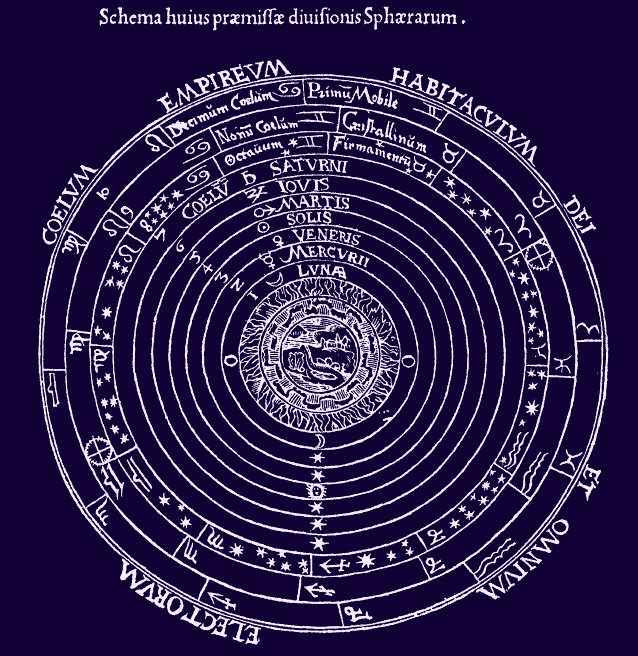
\includegraphics[width=0.4\textwidth]{sphere-medieval.png}\EC
\small
}


\frame{\frametitle{\textbf{Some announcements}}
\Large
If you missed class Tuesday:
\BI
\item{Course website: \url{walterfreeman.github.io/ast101/}}
\item{The syllabus, the {\it Mastering Astronomy} info, etc. is all there}
\item{Course email: suastronomy101@gmail.com}
\item{Extra colored cards will be available each class}
\item{No labs until the third week of class}
\EI
}


\frame{\frametitle{\textbf{Some announcements}}
\Large

On the textbooks:

\large

\BI
\item{Yes, you need the books}
\item{Any edition, paper or electronic, is fine for the text}
\item{You need a paper copy of the {\it Lecture Tutorials}}
\item{I know the Bookstore's out; I will bother them}
\item{If you don't have the {\it Tutorials}, share with a (new) friend today}
\EI
}

\frame{\frametitle{\textbf{Some announcements}}
\Large

On {\it Mastering Astronomy}:

\large

\BI
\item{The course code is on the website: {\tt SUASTRO101FALL2016}}
\item{Access codes: either from the bookstore or purchased separately}
\item{Please give me your feedback about the software}
\EI
}

\frame{\frametitle{\textbf{Some announcements}}
\Large

\begin{center}
I will be out of town on Friday; no help session hours. Sorry!

\bigskip
\bigskip
\bigskip

I will only have a few minutes a day to answer email over the weekend. 
If you email me and it's not extremely urgent, I will answer next week.

\end{center}
}

\frame{\frametitle{\textbf{Some announcements}}
\Large
Lab section changes are tricky because things are very full.

\bigskip
\bigskip
\bigskip

I can't process these (I don't have access). Talk to Patty Whitmore (pawhitmo@syr.edu);
her office is room 111.

\bigskip
\bigskip
\bigskip
}

\frame{\frametitle{\textbf{The night sky and the celestial sphere: overview}}
\Large
\BI
\item{What's the night sky look like?}
\item{How have we affected the night sky?}
\item{How does the night sky move each night?}
\BI
\item{The celestial-sphere model}
\item{Why it works, and when it doesn't}
\item{The first {\it Lecture Tutorial}}
\EI
\EI
}

\frame{\frametitle{\textbf{Virtual planetarium software}}
\Large
We can simulate the night sky tonight using {\it Stellarium}, virtual planetarium software.

\bigskip
\bigskip

It's available for free on Linux, Mac OSX, and Windows.

\normalsize

\BI
\item{Ubuntu users: {\tt sudo apt install stellarium}}
\item{Windows users: see links on {\tt stellarium.org}}
\EI
}


\frame{\frametitle{\textbf{Light pollution}}
\centerline{\large What do you think about this picture?} 

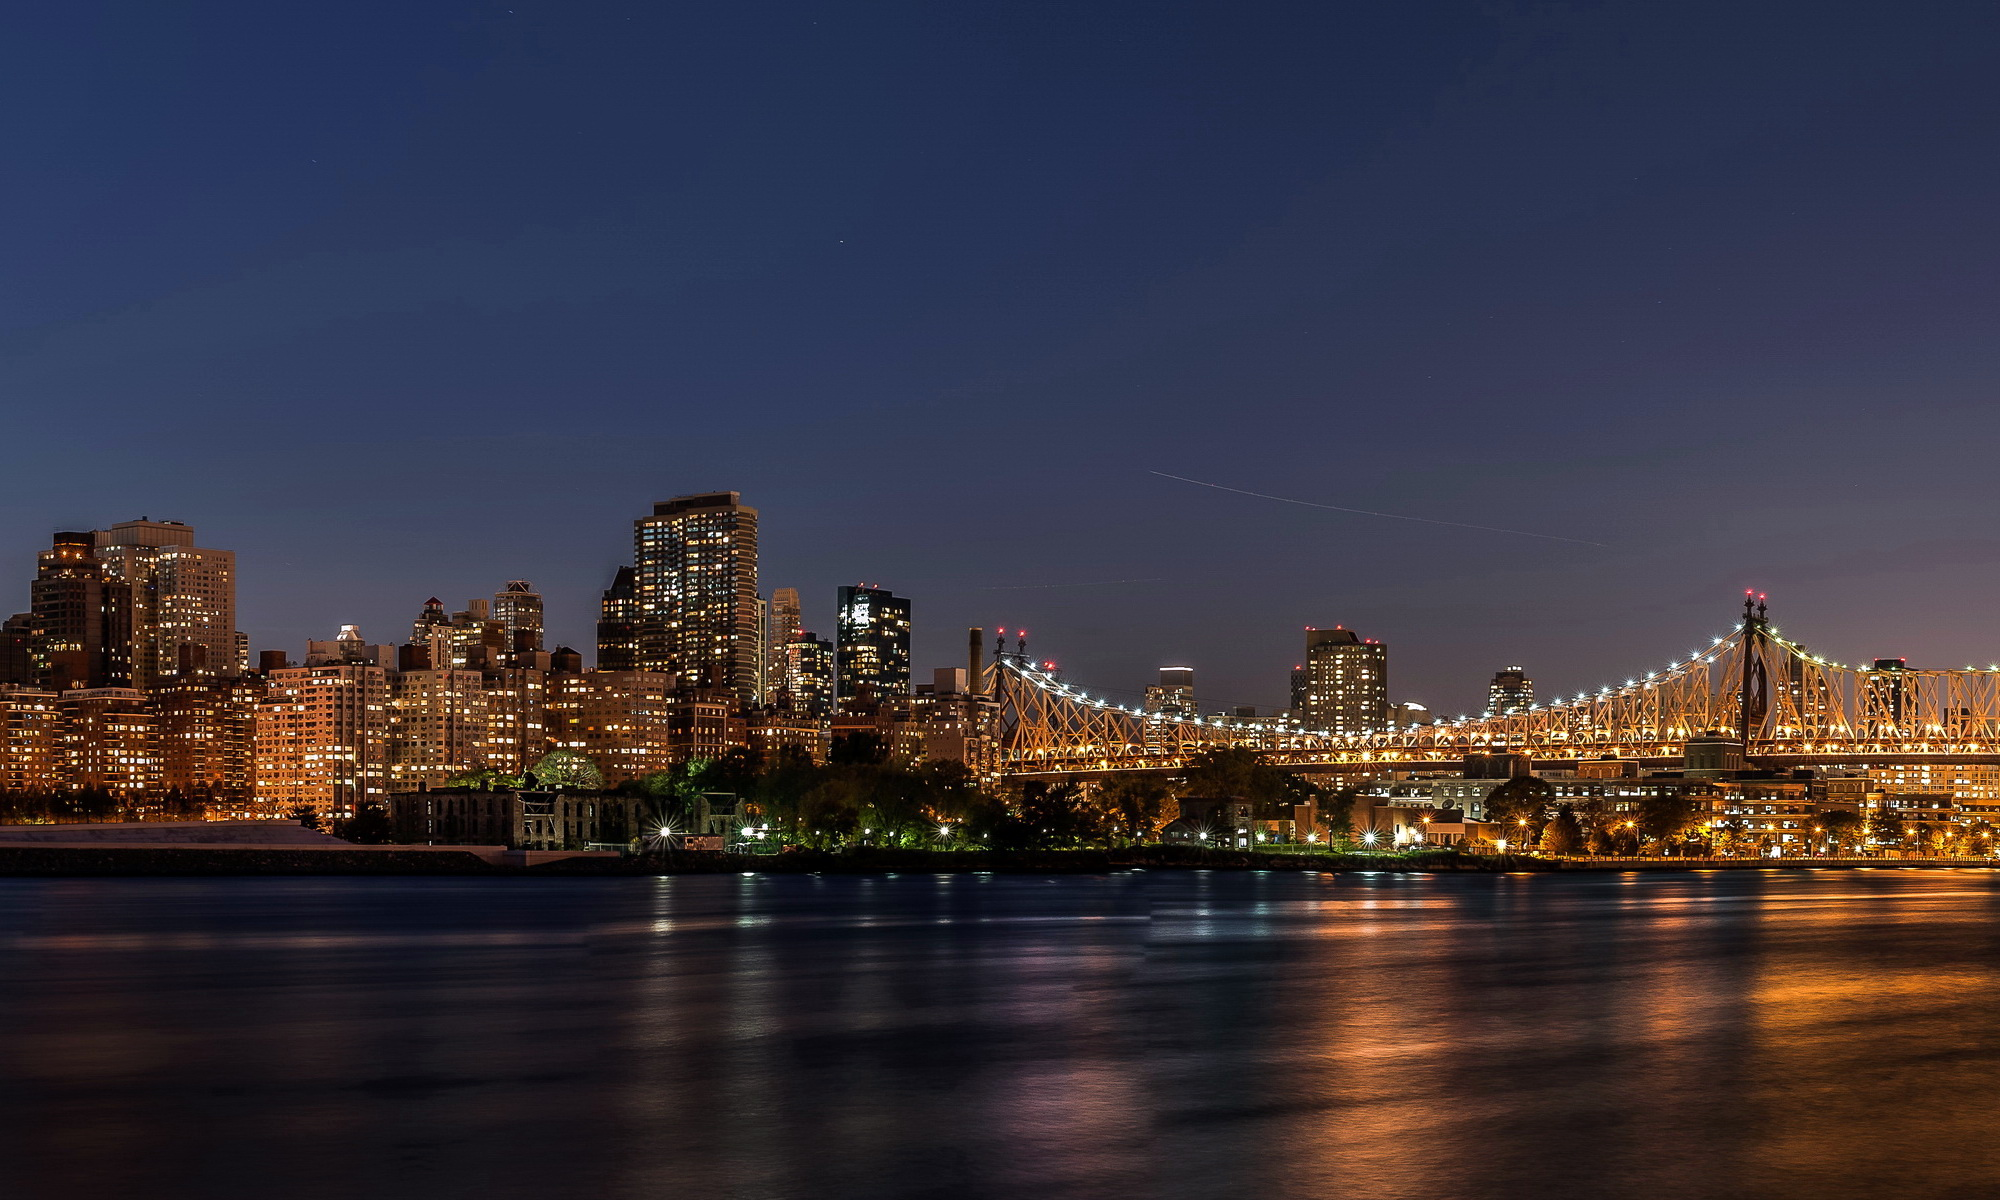
\includegraphics[width=\textwidth]{nyc-skyline.jpg}

}

\frame{\frametitle{\textbf{Light pollution}}
\centerline{\large This is what we could have instead!} 

\begin{center}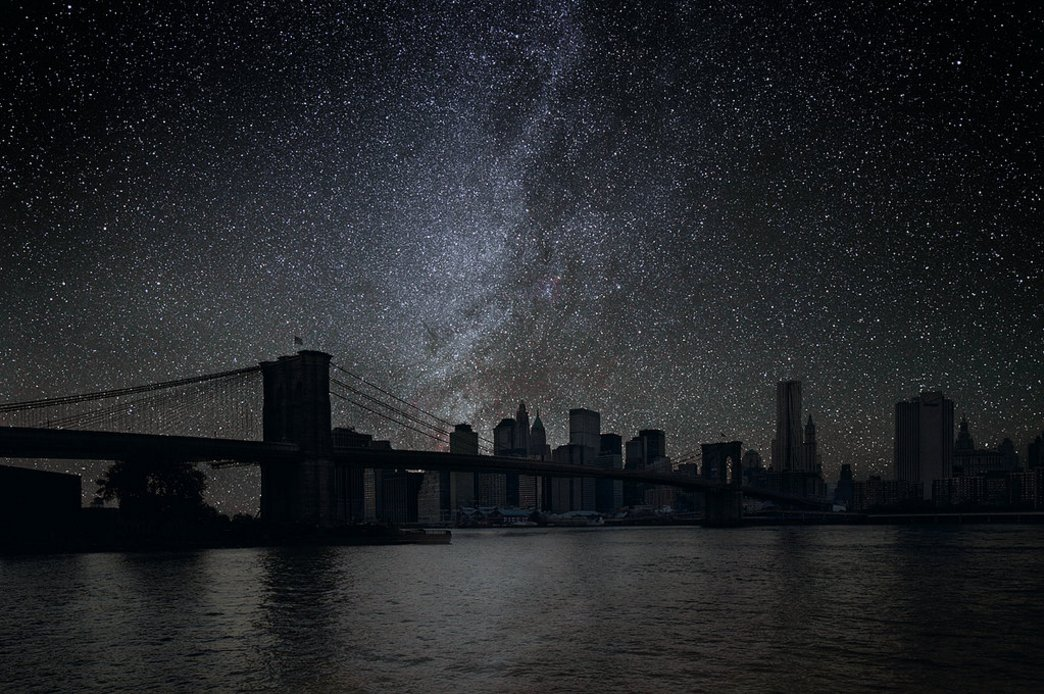
\includegraphics[width=0.95\textwidth]{nyc-skyline-dark.jpg}\end{center}

}

\frame{\frametitle{\textbf{Our disappearing heritage: the night sky}}

The previous image is from the {\it New York Times:} see \url{http://www.nytimes.com/interactive/2013/02/03/magazine/look-stars.html}.

\bigskip
\bigskip
\bigskip

\large We {\it can}, if we try, reclaim this heritage for all of us!
}

\frame{\frametitle{\textbf{Alamut, Iran}}
\BC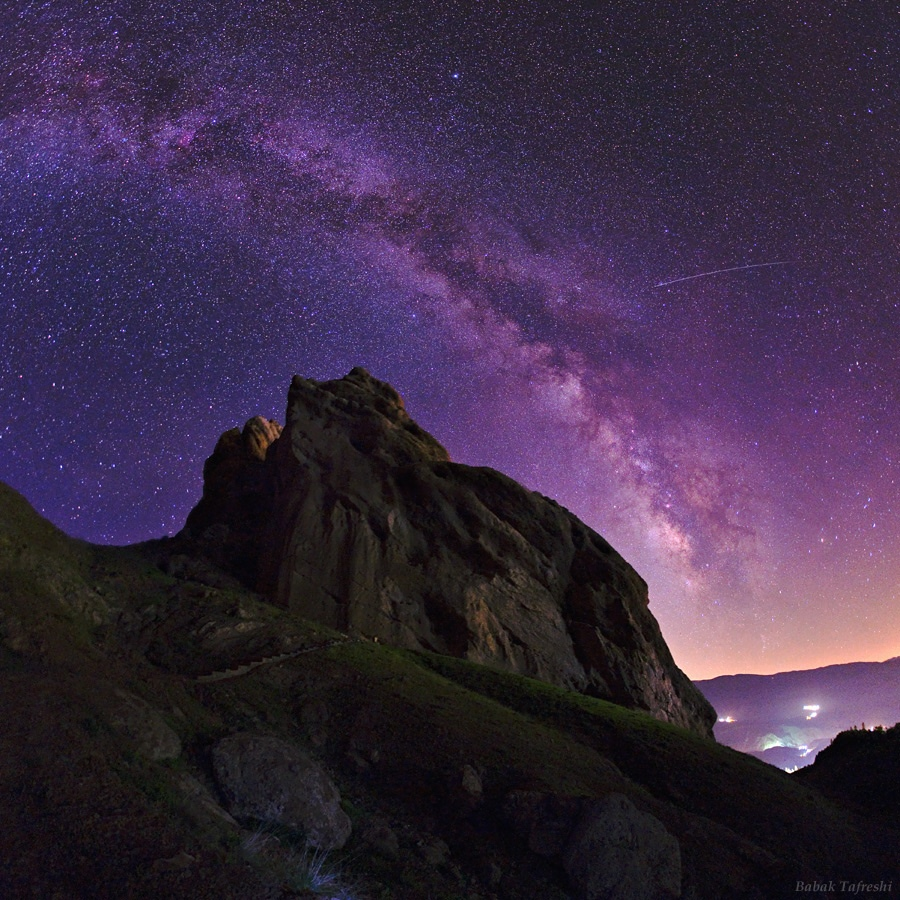
\includegraphics[width=0.6\textwidth]{alamut-babak.jpg}\EC
\small{Photo by Babek Tafreshi. Alamut was the home of Nasir al-Din al-Tusi, the first to surmise that the Milky Way was made of many stars in the $13^{\rm th}$ century. The glow is light pollution from Tehran, 100 km away.}
}

\frame{\frametitle{\textbf{Let's look at the planetarium software again...}}
\Large
How do these stars move? 

\bigskip
\bigskip

\pause

\BC 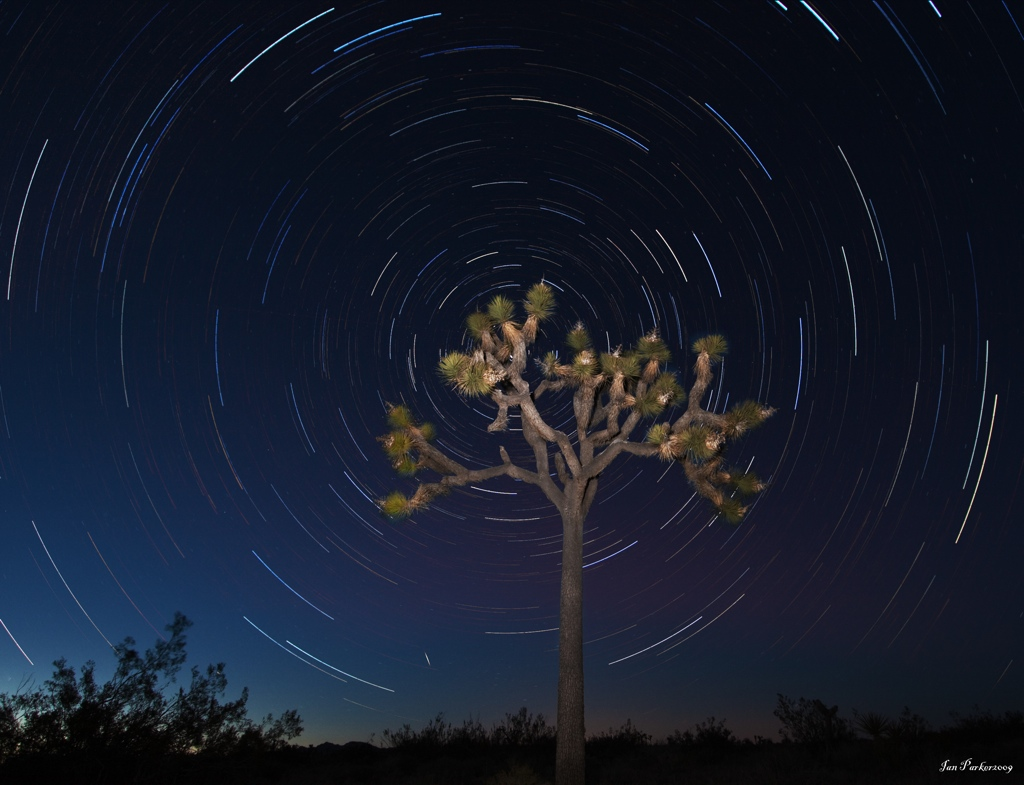
\includegraphics[width=0.55\textwidth]{joshua-tree-circle.jpg}\EC

The ``celestial sphere'' model of Ptolemy:

\BI
\item{All the stars are attached to a sphere, very far away}
\item{This rotates around the Earth, once per day}
\EI
}

\frame{\frametitle{\textbf{A question for you...}}
\Large
How much of the celestial sphere can we see at a time?

\bigskip
\bigskip
\Huge
\color{A}A: All of it \\
\color{B}B: More than half  \\
\color{C}C: Half of it \\
\color{D}D: Less than half \\
\color{E}E: It depends on your latitude \\
}

\frame{\frametitle{\textbf{How good is this ``celestial sphere'' model, anyway?}}
\Large

\color{A}A: It's completely wrong; we know it's not like that! \\ 
\color{B}B: It's pretty close to correct, with a few exceptions \\
\color{C}C: It's correct, just look at the sky! \\ 
\color{D}D: It explains a lot of things, so it must have {\it some} use \\
\pause
\color{E}E: I thought Dr. Freeman was supposed to tell {\it us} this stuff?
}

\frame{\frametitle{\textbf{Problems with the celestial sphere: I}}

\Large

\BC Discuss with your neighbors: what's wrong with the celestial sphere? \EC

\pause \bigskip \bigskip

Is it really true that {\it every} star in the sky moves in the same way, all together?

\pause \bigskip \bigskip

Actually, (--------) rotates, and (--------) doesn't move much at all.
}

\frame{\frametitle{\textbf{Problems with the celestial sphere: II}}

\Large

Is it really true that all the stars are stuck to a sphere, all at the same distance from us? 

\pause \bigskip \bigskip

No; we just don't have any ``depth perception'' of things this far away.
}

\frame{\frametitle{\textbf{Depth and the sky}}
\BC \Large The constellation of Orion:\EC

\begin{columns}
\begin{column}{0.5\textwidth}
\BC 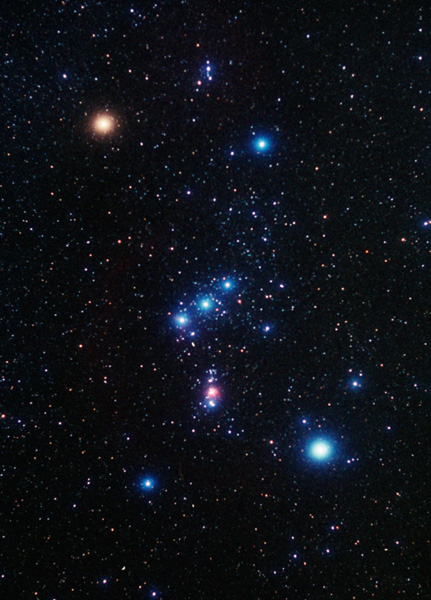
\includegraphics[width=0.8\textwidth]{orion-flat.jpg}\EC
\end{column}
\pause
\begin{column}{0.5\textwidth}
\BC 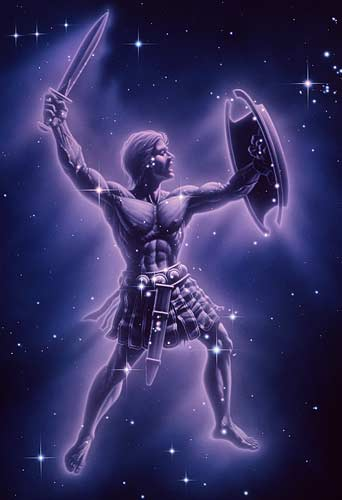
\includegraphics[width=0.8\textwidth]{orion-art.jpg}\EC
\end{column}`
\end{columns}
}

\frame{\frametitle{\textbf{Depth and the sky}}
\BC \Large The reality:\EC

\bigskip
\bigskip

\BC 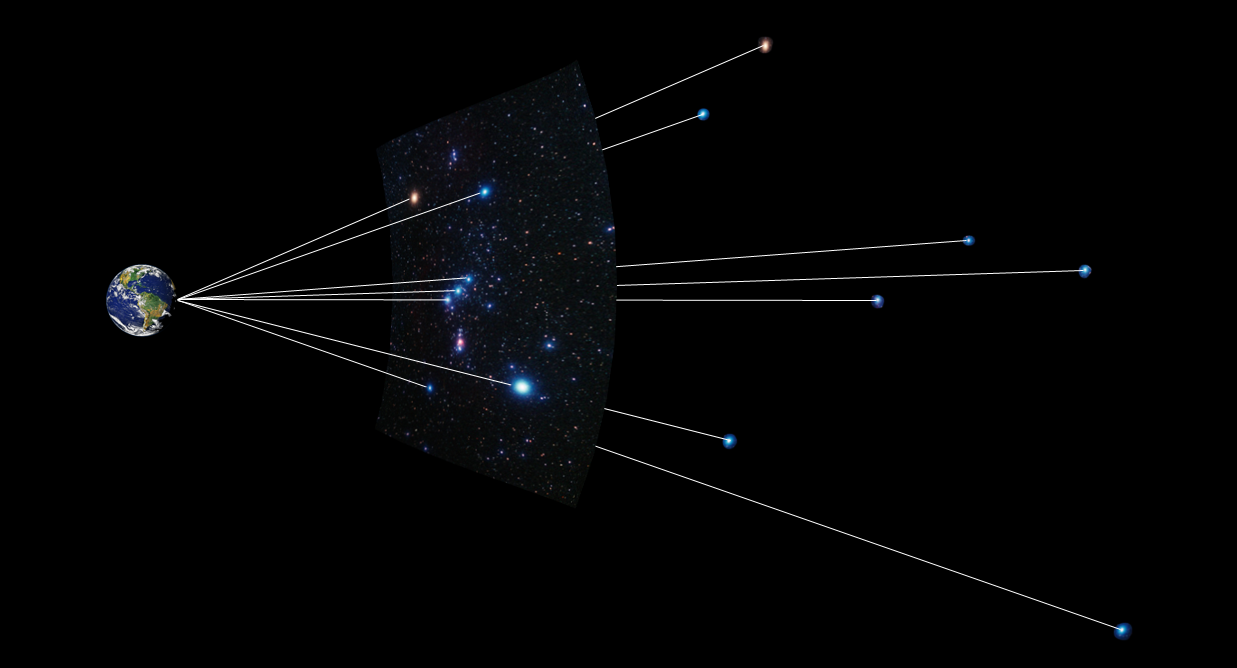
\includegraphics[width=0.9\textwidth]{orion-depth.png}\EC
}

\frame{\frametitle{\textbf{Why the celestial sphere still explains a lot}}
\Large
Key idea \#1: the stars are {\color{Red}very far away} compared to the Earth's motion!
\Large
\BI
\item{Parallax experiment: try it!}
\pause
\item{It doesn't matter that the stars are different distances away}
\item{... since those distances are so huge compared to our motion}
\pause
\item{\color{Red}This means that the celestial sphere's predictions will be {\it badly wrong} for the motion of the Sun and the planets!}
\EI

\pause
\bigskip
\bigskip

Key idea \#2: It doesn't matter if Earth rotates or the celestial sphere rotates: {\color{Red}relative} motion controls what we see! 

\BI
\item{The celestial sphere model is just dizzy!}
\EI
}

\frame{\frametitle{\textbf{Summary}}
\large
\BI
\item{We can treat the stars as all rotating together, on an invisible sphere far away}
\item{We expect this to get the stars ``right'' and the planets and Sun ``wrong''}
\item{The axis of rotation is the same as the Earth's, and it rotates once per day}
\item{Only half of the sphere is visible, because the Earth is in the way}
\item{{\color{Red} Horizon:} a plane lying along the Earth at our location}
\item{{\color{Red} Zenith:} the point directly overhead}
\item{{\color{Red} Celestial pole:} the point about which the stars appear to rotate}
\EI
\begin{columns}
\begin{column}{0.5\textwidth}
\BC
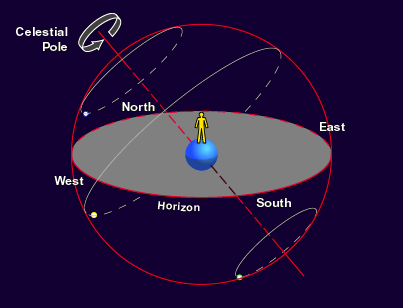
\includegraphics[width=0.8\textwidth]{sphere-1.png}\EC \end{column}
\begin{column}{0.5\textwidth}
\BC
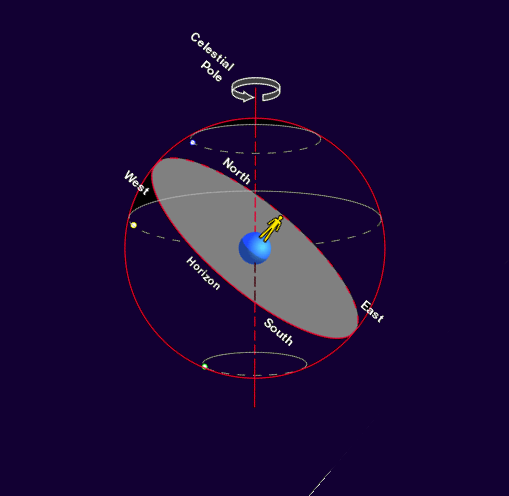
\includegraphics[width=\textwidth]{sphere-2.png}
\EC 
\end{column}
\end{columns}
}

\frame{\frametitle{\textbf{How many celestial poles are there?}}
\begin{columns}
\begin{column}{0.4\textwidth}
\Huge
\color{A}A: One \\
\color{B}B: Two \\
\color{C}C: Three \\
\color{D}D: Four 
\end{column}
\pause
\begin{column}{0.6\textwidth}
\BC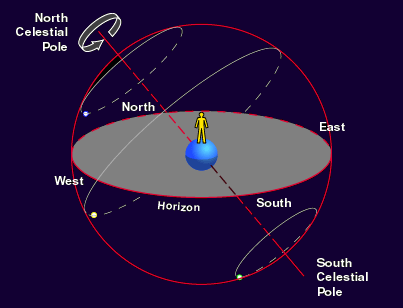
\includegraphics[width=0.8\textwidth]{sphere-3.png}\EC 
\end{column}
\end{columns}
}

\frame{\frametitle{\textbf{Summary}}
\large
\BI
\item{We can treat the stars as all rotating together, on an invisible sphere far away}
\item{We expect this to get the stars ``right'' and the planets and Sun ``wrong''}
\item{The axis of rotation is the same as the Earth's, and it rotates once per day}
\item{Only half of the sphere is visible, because the Earth is in the way}
\item{{\color{Red} Horizon:} a plane lying along the Earth at our location}
\item{{\color{Red} Zenith:} the point directly overhead}
\item{{\color{Red} Celestial poles:} the points about which the stars appear to rotate}
\EI
\BC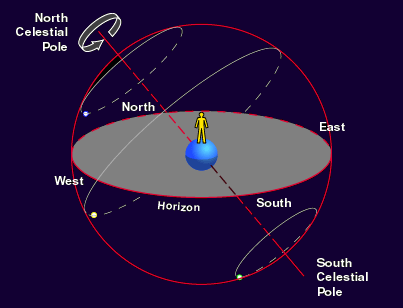
\includegraphics[width=0.5\textwidth]{sphere-3.png}\EC 
}

\frame{\frametitle{\textbf{Lecture tutorials}}
\Huge
\BC
Complete pages 1-4 (``Part I'')
\EC
}

\frame{\frametitle{\textbf{Which are true in Syracuse?}}
\Large
\BI
\item{I: Some stars are always visible (at night).}
\item{II: Some stars are only visible sometimes; they rise and set during the night}
\item{III: Some stars are never visible}
\EI

\bigskip
\bigskip

\color{A}A: I only \\
\color{B}B: II only \\
\color{C}C: III only \\
\color{D}D: I and II \\
\color{E}E: I, II, and III 
}

\frame{\frametitle{\textbf{What is this?}}
\BC
\includegraphics[width=0.6\textwidth]{aus-flag.png}\EC

\pause

\Large \BC The Australian flag, with a pattern of stars called the Southern Cross.

These stars are only visible in the Southern Hemisphere!
\EC
}

\frame{\frametitle{\textbf{For next time:}}
\huge
\BI
\item{Visit the course webpage}
\item{Complete the first Mastering Astronomy assignment}
\item{Read pp. 25-32 of your text if you haven't already}
\item{Look up!}
\EI

\bigskip
\bigskip



}

\end{document}
